\section{Controlador de Video}
$\mu$VGA PICASO-MD1 es un motor de gr\'aficos que por medio de comandos integrados, nos permite desde poner un color de fondo hasta producir una gran variedad de formas y tama\~nos que pueden incluir caracteres de mapas de bits definibles por el usuario. Sus principales caracter\'isticas son:\medskip

\begin{itemize}
\item Controlador gr\'afico VGA / SVGA inteligente y completamente integrado.

\item Reducido m\'odulo 28 pines, alimentado por el chip PICASO de 4D LABS. Un poderoso motor DSP/Contralor de m\'ultiples efectos gr\'aificos.

\item Dise\~no de bajo consumo. De 3.0 Voltios a 3.6Volts @ 90ma para alimentarlo.

\item 256K colores con resoluci\'on est\'andar para modos QVGA (320x240), VGA (640x480), y SVGA (800x600, que se realizar\'an proximamente). La $\mu$VGA PICASO-MD1 soporta m\'ultiples resoluciones con el mismo m\'odulo. Las distintas resoluciones son seleccionables durante la ejecuci\'on bajo el control de Host. Permite reescalado de la visualización de ventanas parcial/pantalla completa.

\item Las se\~nales digitales de v\'ideo, RED0: RED2, GREEN0: GREEN2, BLUE1: BLUE2, HSYNC, VSYNC and BLANK(R,G,B), facilitadas usando un simple resistor-DAC para manejar cualquier monitor VGA estándar.

\item 512K bytes de SRAM a de memoria de video incluidos permite 8 p\'aginas para QVGA, 2 p\'aginas para VGA y 1 p\'agina para resoluciones SVGA. La utilizaci\'on de las m\'ultiples p\'aginas permite doble buffer que puede ser usado para animaciones planas y ventanas de los sistemas de men\'u.

\item Se\~nales RX y TX (niveles TTL) proporcionan una sencilla interfaz de serie de acogida. La interfaz serie permite al m\'odulo de gr\'aficos $\mu$VGA PICASO-MD1 ser conectado a cualquier controlador como un PIC, AVR, SELLO, ARM, Propeller solo por nombrar a unos cuantos, as\'i como una PC. El anfitri\'on controla el m\'odulo mediante el env\'io de comandos simples serie. Auto detecci\'on de la tasa de baudios 2400 baudios a 1Mbit/sec.

\item De gran alcance, potente y f\'acil de utilizar y entender, con funciones integradas que permiten dibujar gr\'aficos de l\'ineas, rect\'angulos, c\'irculos, elipses, texto, im\'agenes, iconos, mapas de bits definidos por el usuario y mucho m\'as ...
\end{itemize}

Con este controlador se manejara la parte del video en 2-Dimensiones para el microprocesador, la primera fase consiste en la integraci\'on del controlador gr\'afico realizando pruebas para familiarizarnos con los comandos internos, para posteriormente poder integrarlo en el simulador. Todas las pruebas se realizaran con la ayuda del lenguaje de programaci\'on PYTHON debido a la facilidad con la que podemos mandar informaci\'on serial. Una limitaci\'on importante fue que las computadoras actuales no cuentan con puerto serial y toda la comunicaci\'on con el controlador gr\'afico es por medio de este puerto, para solucionar el problema se necesita simular un puerto serial a traves del USB, para esto usamos un FTDI(FT232RL). En la figura~\ref{fig:serie} se puede observar la forma en la que conectamos las placas para la realizaci\'on de las pruebas.\medskip

\begin{figure}[H]
\centering
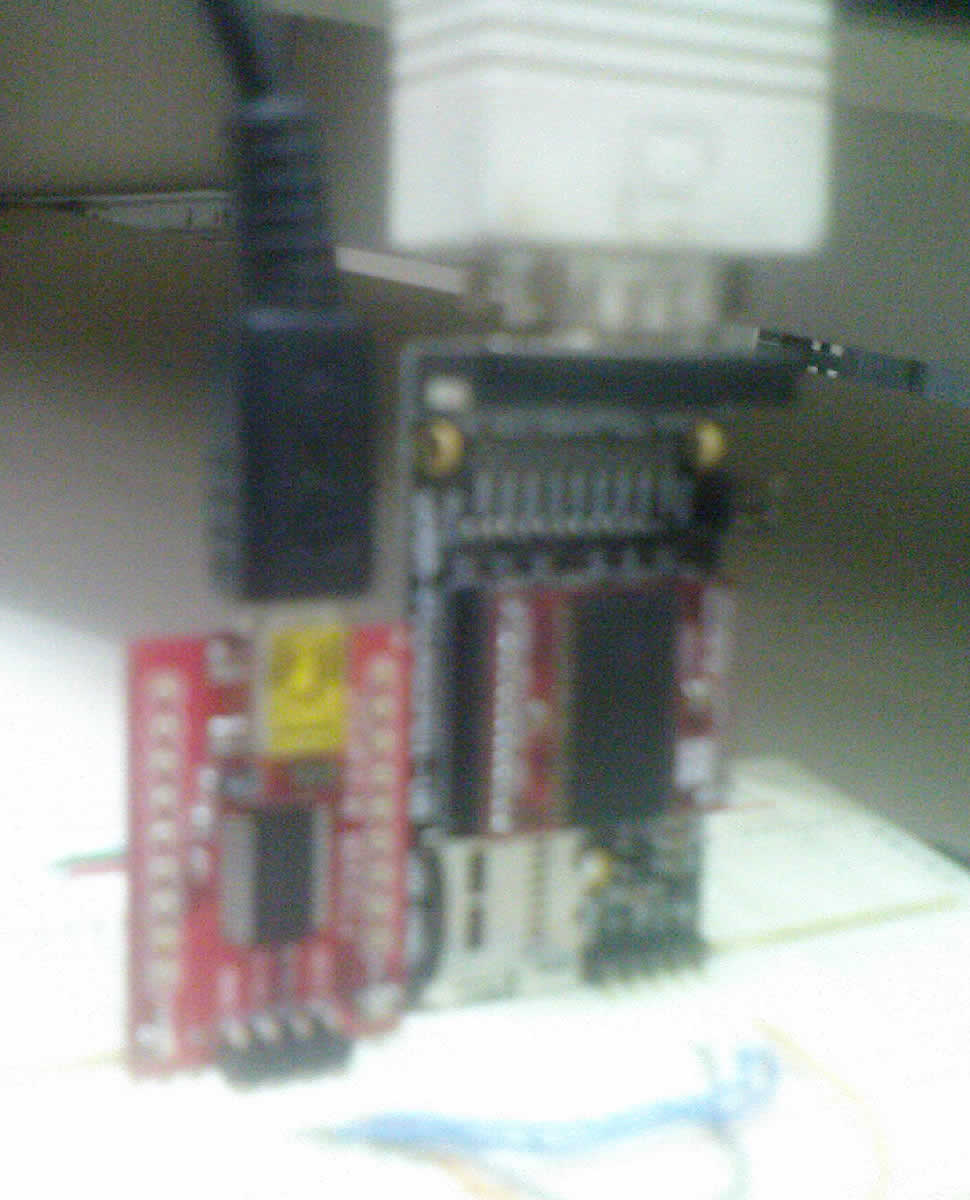
\includegraphics[scale=0.1]{serie}
\caption{Conexi\'on  de las placas para la comunicaci\'on PC-PICASO-MONITOR}\label{fig:serie}
\end{figure}

Para la primera prueba (figura~\ref{fig:fcirculo}) se planteo poner un color de fondo y colocar una figura b\'asica como el c\'irculo.\medskip

\begin{figure}[H]
\centering
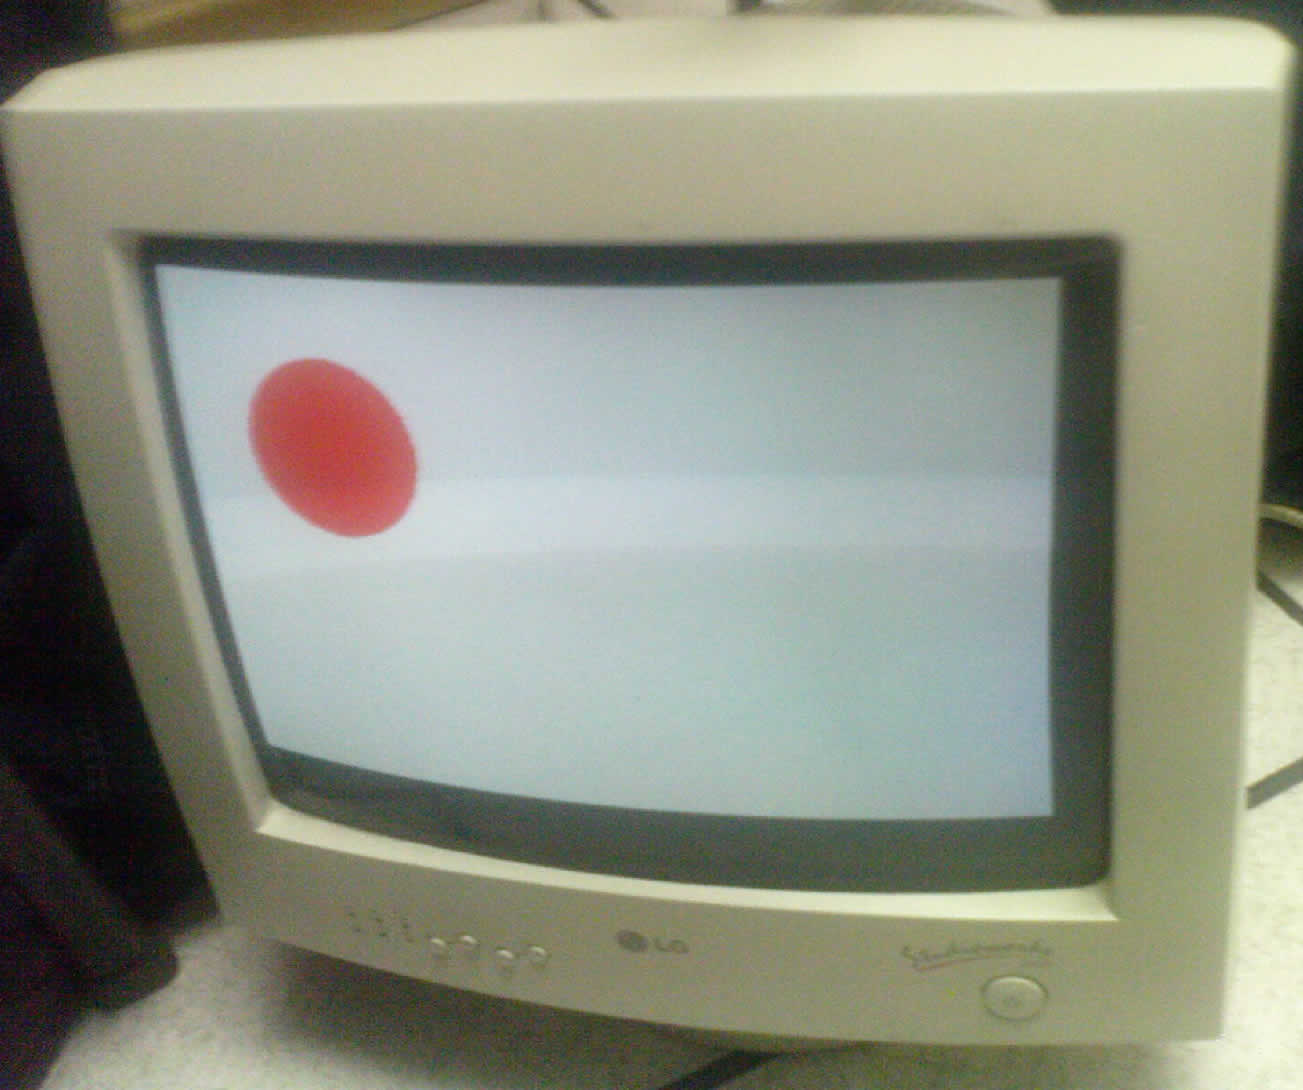
\includegraphics[scale=0.1]{fcirculo}
\caption{Fondo blanco y c\'irculo rojo}\label{fig:fcirculo}
\end{figure}

La segunda prueba consiste en mandar una imagen (.bmp) y modificar la resoluci\'on de la pantalla ya que por default se tiene QVGA. En la figura~\ref{fig:prueba} se muestran todas las fases por las que se paso para que la segunda prueba quedara finalizada.\medskip

\begin{figure}[H]
\centering
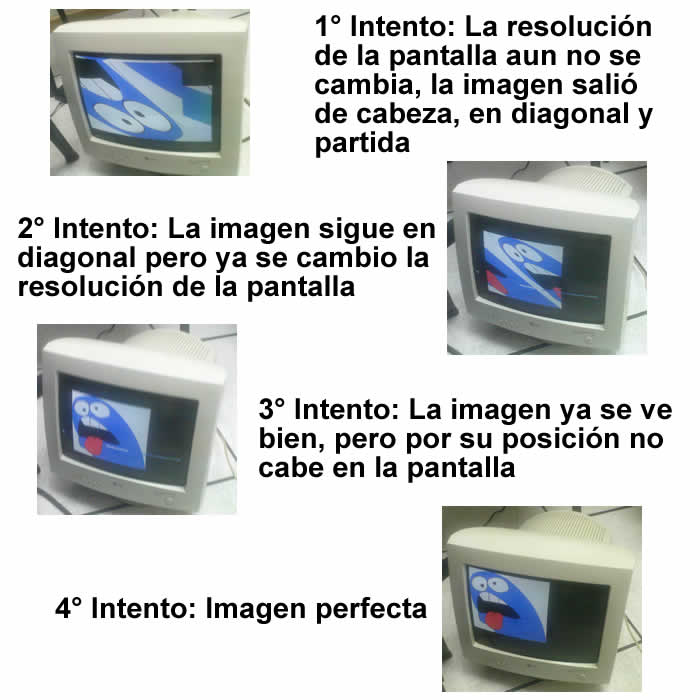
\includegraphics[scale=0.5]{prueba}
\caption{Conjunto de intentos para la segunda prueba}\label{fig:prueba}
\end{figure}

El codigo en PYTHON con el cual logramos cargar la imagen es el siguiente:

\lstset{language=PYTHON}
\lstinputlisting{./img.py}

En el c\'odigo anterior podemos observar que se obtiene toda la informaci\'on de la imagen .bmp que se pasa como par\'ametro al programa en PYTHON, esta informaci\'on nos sirve para saber las dimensiones de la imagen, asi como su tipo. La imagen debe de tener m\'aximo 8 bits o un byte por pixel. Y tambi\'en se puede observar como se configura la resoluci\'on de la pantalla.
